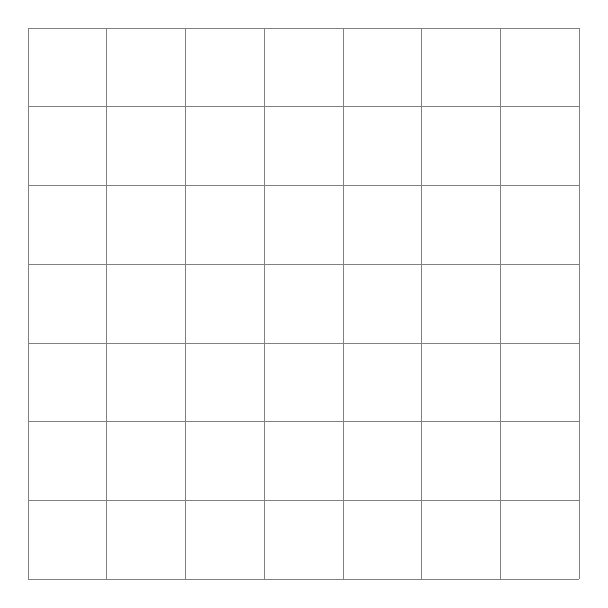
\begin{tikzpicture} 
	\draw [help lines] (0,0) grid (7,7) ;
\end{tikzpicture}

\tikzset{every node/.append style={font=\sffamily}}

\begin{tikzpicture}[help lines/.append style={step=5mm}]
    \draw [help lines] (0,0) grid (7,10) ;
    \filldraw[fill=gray!20, draw=black,very thick]  
        (1,1) rectangle node [fill=blue!10,draw=black,inner sep=10pt] {окно} +(5,5) 
        coordinate (ПравоВерх);
     \filldraw [fill=red!30] (ПравоВерх)   +(1,0) -- +(-2.5,2)  -- +(-6,0)  --cycle  ;
        
\end{tikzpicture}
